% Options for packages loaded elsewhere
\PassOptionsToPackage{unicode}{hyperref}
\PassOptionsToPackage{hyphens}{url}
\PassOptionsToPackage{dvipsnames,svgnames,x11names}{xcolor}
%
\documentclass[
  beamerpaper,
  DIV=11,
  numbers=noendperiod,
  aspectratio=54]{scrreprt}

\usepackage{amsmath,amssymb}
\usepackage{iftex}
\ifPDFTeX
  \usepackage[T1]{fontenc}
  \usepackage[utf8]{inputenc}
  \usepackage{textcomp} % provide euro and other symbols
\else % if luatex or xetex
  \usepackage{unicode-math}
  \defaultfontfeatures{Scale=MatchLowercase}
  \defaultfontfeatures[\rmfamily]{Ligatures=TeX,Scale=1}
\fi
\usepackage{lmodern}
\ifPDFTeX\else  
    % xetex/luatex font selection
  \setmonofont[Scale=0.6]{Source Code Pro}
\fi
% Use upquote if available, for straight quotes in verbatim environments
\IfFileExists{upquote.sty}{\usepackage{upquote}}{}
\IfFileExists{microtype.sty}{% use microtype if available
  \usepackage[]{microtype}
  \UseMicrotypeSet[protrusion]{basicmath} % disable protrusion for tt fonts
}{}
\makeatletter
\@ifundefined{KOMAClassName}{% if non-KOMA class
  \IfFileExists{parskip.sty}{%
    \usepackage{parskip}
  }{% else
    \setlength{\parindent}{0pt}
    \setlength{\parskip}{6pt plus 2pt minus 1pt}}
}{% if KOMA class
  \KOMAoptions{parskip=half}}
\makeatother
\usepackage{xcolor}
\setlength{\emergencystretch}{3em} % prevent overfull lines
\setcounter{secnumdepth}{-\maxdimen} % remove section numbering
% Make \paragraph and \subparagraph free-standing
\ifx\paragraph\undefined\else
  \let\oldparagraph\paragraph
  \renewcommand{\paragraph}[1]{\oldparagraph{#1}\mbox{}}
\fi
\ifx\subparagraph\undefined\else
  \let\oldsubparagraph\subparagraph
  \renewcommand{\subparagraph}[1]{\oldsubparagraph{#1}\mbox{}}
\fi


\providecommand{\tightlist}{%
  \setlength{\itemsep}{0pt}\setlength{\parskip}{0pt}}\usepackage{longtable,booktabs,array}
\usepackage{calc} % for calculating minipage widths
% Correct order of tables after \paragraph or \subparagraph
\usepackage{etoolbox}
\makeatletter
\patchcmd\longtable{\par}{\if@noskipsec\mbox{}\fi\par}{}{}
\makeatother
% Allow footnotes in longtable head/foot
\IfFileExists{footnotehyper.sty}{\usepackage{footnotehyper}}{\usepackage{footnote}}
\makesavenoteenv{longtable}
\usepackage{graphicx}
\makeatletter
\def\maxwidth{\ifdim\Gin@nat@width>\linewidth\linewidth\else\Gin@nat@width\fi}
\def\maxheight{\ifdim\Gin@nat@height>\textheight\textheight\else\Gin@nat@height\fi}
\makeatother
% Scale images if necessary, so that they will not overflow the page
% margins by default, and it is still possible to overwrite the defaults
% using explicit options in \includegraphics[width, height, ...]{}
\setkeys{Gin}{width=\maxwidth,height=\maxheight,keepaspectratio}
% Set default figure placement to htbp
\makeatletter
\def\fps@figure{htbp}
\makeatother

\usepackage{titling}
\usepackage{fancyhdr, blindtext}
\usepackage{xcolor}
\usepackage{soul}
\usepackage{pagecolor}
\usepackage{booktabs}
\usepackage{longtable}
\usepackage{array}
\usepackage{multirow}
\usepackage{wrapfig}
\usepackage{float}
\usepackage{colortbl}
\usepackage{pdflscape}
\usepackage{tabu}
\usepackage{threeparttable}
\usepackage{threeparttablex}
\usepackage[normalem]{ulem}
\usepackage{makecell}
\usepackage{tcolorbox}
\usepackage[]{Oswald}
\usepackage{lipsum}

\definecolor{merkgreen}{RGB}{202,211,68}
\definecolor{merkdarkgreen}{RGB}{52,93,70}
\definecolor{merkyellow}{RGB}{247,233,9}

\definecolor{bggray}{rgb}{0.95,0.95,0.95}
\pagestyle{fancy}
\pretitle{\begin{center}
  
\includegraphics[width=5in,height=3.5in]{../../img/logo_Merkanzia.pdf}\LARGE\\}
  \pagecolor{merkdarkgreen}
\posttitle{\end{center}}
\fancyhf{}
\newpage
\newpagecolor{merkgreen}
% \begin{tcolorbox}[
%     title="Prezzi",
% %   opacityback=1,  % this does not work
% %   colback=white,  % this is not what I want
% ]
\fancyfoot[R]{\footnotesize \textit{www.merkanzia.com info@merkanzia.com}}
\fancyfoot[L]{\footnotesize \textit{Merkanzia GmbH, La Toscana in Svizzera}}
\usepackage{booktabs}
\usepackage{longtable}
\usepackage{array}
\usepackage{multirow}
\usepackage{wrapfig}
\usepackage{float}
\usepackage{colortbl}
\usepackage{pdflscape}
\usepackage{tabu}
\usepackage{threeparttable}
\usepackage{threeparttablex}
\usepackage[normalem]{ulem}
\usepackage{makecell}
\usepackage{xcolor}
\KOMAoption{captions}{tableheading}
\makeatletter
\makeatother
\makeatletter
\makeatother
\makeatletter
\@ifpackageloaded{caption}{}{\usepackage{caption}}
\AtBeginDocument{%
\ifdefined\contentsname
  \renewcommand*\contentsname{Table of contents}
\else
  \newcommand\contentsname{Table of contents}
\fi
\ifdefined\listfigurename
  \renewcommand*\listfigurename{List of Figures}
\else
  \newcommand\listfigurename{List of Figures}
\fi
\ifdefined\listtablename
  \renewcommand*\listtablename{List of Tables}
\else
  \newcommand\listtablename{List of Tables}
\fi
\ifdefined\figurename
  \renewcommand*\figurename{Figure}
\else
  \newcommand\figurename{Figure}
\fi
\ifdefined\tablename
  \renewcommand*\tablename{Table}
\else
  \newcommand\tablename{Table}
\fi
}
\@ifpackageloaded{float}{}{\usepackage{float}}
\floatstyle{ruled}
\@ifundefined{c@chapter}{\newfloat{codelisting}{h}{lop}}{\newfloat{codelisting}{h}{lop}[chapter]}
\floatname{codelisting}{Listing}
\newcommand*\listoflistings{\listof{codelisting}{List of Listings}}
\makeatother
\makeatletter
\@ifpackageloaded{caption}{}{\usepackage{caption}}
\@ifpackageloaded{subcaption}{}{\usepackage{subcaption}}
\makeatother
\makeatletter
\@ifpackageloaded{tcolorbox}{}{\usepackage[skins,breakable]{tcolorbox}}
\makeatother
\makeatletter
\@ifundefined{shadecolor}{\definecolor{shadecolor}{rgb}{.97, .97, .97}}
\makeatother
\makeatletter
\makeatother
\makeatletter
\makeatother
\ifLuaTeX
  \usepackage{selnolig}  % disable illegal ligatures
\fi
\IfFileExists{bookmark.sty}{\usepackage{bookmark}}{\usepackage{hyperref}}
\IfFileExists{xurl.sty}{\usepackage{xurl}}{} % add URL line breaks if available
\urlstyle{same} % disable monospaced font for URLs
\hypersetup{
  pdftitle={Catalogo Prodotti e Prezzi},
  colorlinks=true,
  linkcolor={blue},
  filecolor={Maroon},
  citecolor={Blue},
  urlcolor={Blue},
  pdfcreator={LaTeX via pandoc}}

\title{Catalogo Prodotti e Prezzi}
\usepackage{etoolbox}
\makeatletter
\providecommand{\subtitle}[1]{% add subtitle to \maketitle
  \apptocmd{\@title}{\par {\large #1 \par}}{}{}
}
\makeatother
\subtitle{Merkanzia GmbH - La Toscana in Svizzera}
\author{}
\date{November 30, 2023\\
\strut \\
\strut \\
info@merkanzia.com}

\begin{document}
\maketitle
\ifdefined\Shaded\renewenvironment{Shaded}{\begin{tcolorbox}[interior hidden, borderline west={3pt}{0pt}{shadecolor}, enhanced, sharp corners, breakable, frame hidden, boxrule=0pt]}{\end{tcolorbox}}\fi

\renewcommand{\arraystretch}{1.6}

\hypertarget{catalogo-prezzi-b2b}{%
\chapter{Catalogo Prezzi B2B}\label{catalogo-prezzi-b2b}}

Merkanzia è la vostra porta d'accesso al cuore della tradizione
culinaria toscana.

Il Catalogo dei prodotti con i rispettivi prodotti e prezzi di
Merkanzia.

La nostra missione è portare in Svizzera prodotti di altissima qualità
provenienti da piccoli produttori artigianali che onorano le più antiche
tradizioni dell'artigianato alimentare toscano.

Con Merkanzia, potrete assaporare i sapori autentici della Toscana,
prodotti con amore da chi ha un profondo rispetto per il suo patrimonio
culinari.

Formaggi, insaccati, sughi per primi piatti tipici toscani, le zuppe
famose della tradizione contadina, dolci e tanto altro.

\begin{figure}

{\centering 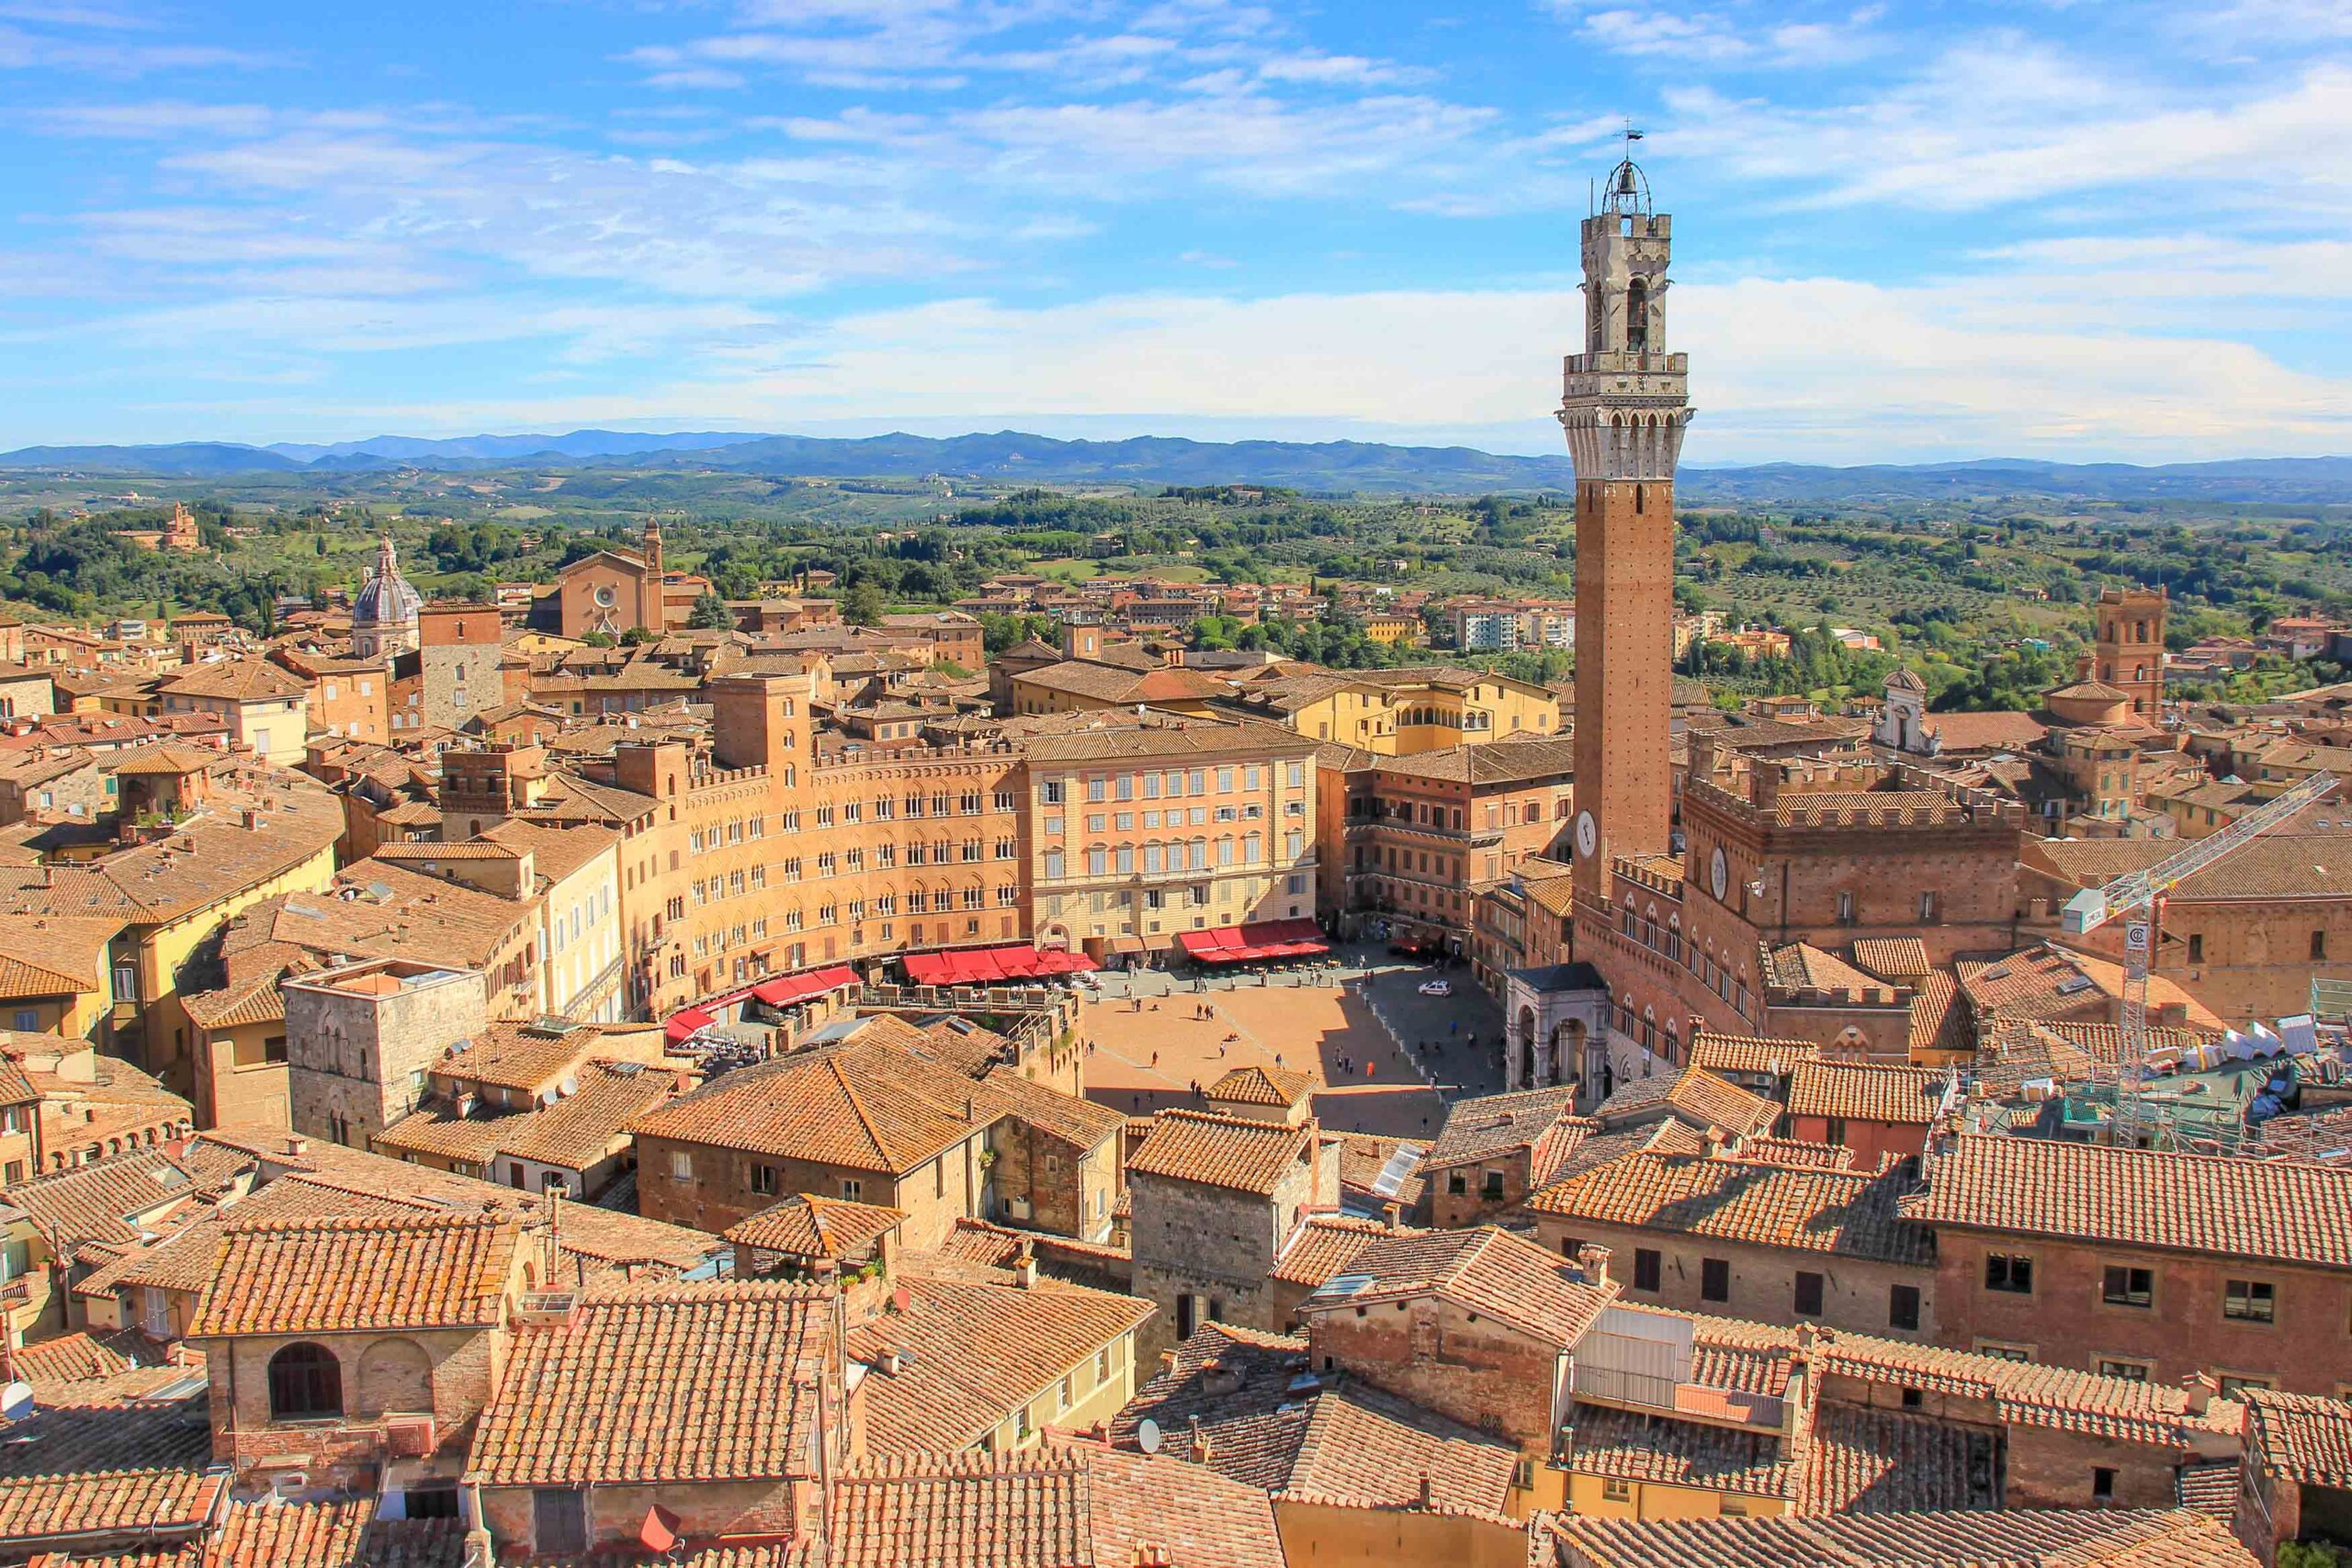
\includegraphics{../../img/Siena-n-1-scaled.jpg}

}

\caption{Siena.}

\end{figure}

\begin{table}

\caption{\label{tbl-panel-cla-aro}Caseificio La Fonte (Asciano -
Siena)}\begin{minipage}[t]{0.60\linewidth}
\subcaption{\label{tbl-panel-cla-aro-1}I Classici }

\tabularnewline

\fontsize{9.5}{11.5}\selectfont
\begin{tabular}{>{\raggedright\arraybackslash}p{3.25cm}>{\raggedright\arraybackslash}p{2.25cm}l}
\toprule
\textbf{Prodotto} & \textbf{Quantità} & \textbf{CHF/Kg}\\
\midrule
\textbf{\em{I Classici di La Fonte}} & \textbf{Una forma 1,5 kg} & \textbf{}\\
\cmidrule{1-3}
 & < 10 kg & 35.6\\

\multirow[t]{-2}{3.25cm}{\raggedright\arraybackslash \em{Sua Eccellenza il Fresco (20gg)}} & > 10kg & 32.1\\
\cmidrule{1-3}
 & < 10 kg & 32.6\\

\multirow[t]{-2}{3.25cm}{\raggedright\arraybackslash \em{Sua Eccellenza il Semi Stagionato (60gg)}} & > 10kg & 29.4\\
\cmidrule{1-3}
 & < 10 kg & 38\\

\multirow[t]{-2}{3.25cm}{\raggedright\arraybackslash \em{Sua Eccellenza lo Stagionato (90gg)}} & > 10kg & 34.2\\
\bottomrule
\multicolumn{3}{l}{\rule{0pt}{1em}\textit{Note: }}\\
\multicolumn{3}{l}{\rule{0pt}{1em}gg: Giorni Stagionatura}\\
\multicolumn{3}{l}{\rule{0pt}{1em}}\\
\end{tabular}

\end{minipage}%
%
\begin{minipage}[t]{0.40\linewidth}

\raisebox{-\height}{

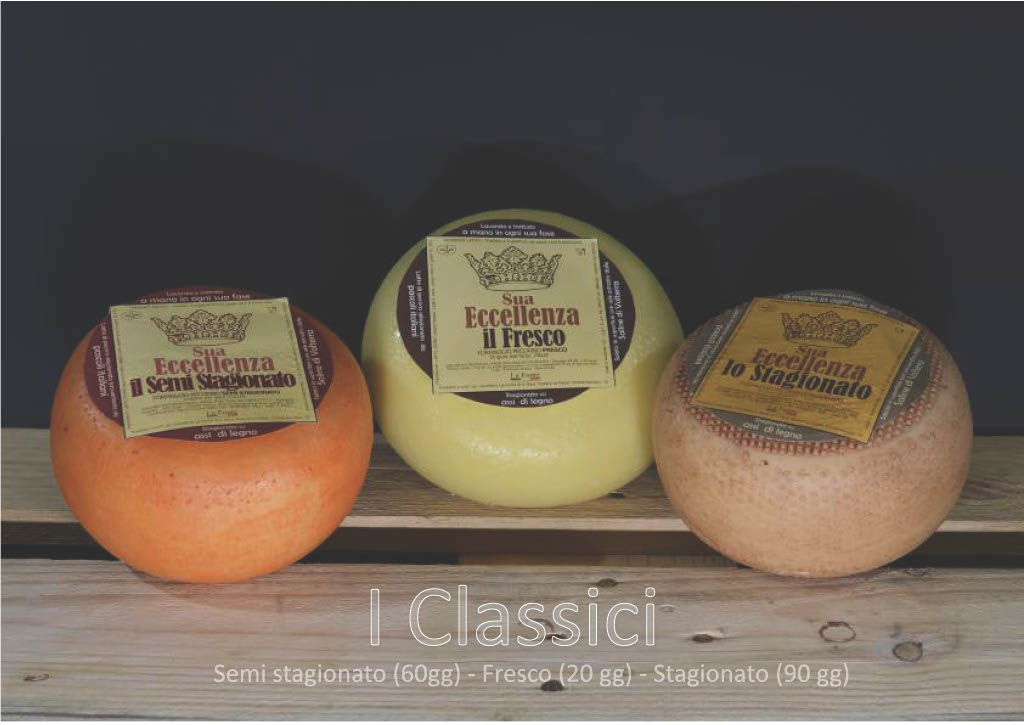
\includegraphics{../../img/LaFonte_IClassici1024_1.jpeg}

}

\end{minipage}%
\newline
\begin{minipage}[t]{0.60\linewidth}
\subcaption{\label{tbl-panel-cla-aro-2}Gli Aromatizzati }

\tabularnewline

\fontsize{9.5}{11.5}\selectfont
\begin{tabular}{>{\raggedright\arraybackslash}p{3.25cm}>{\raggedright\arraybackslash}p{2.25cm}l}
\toprule
\textbf{Prodotto} & \textbf{Quantità} & \textbf{CHF/Kg}\\
\midrule
\textbf{\em{Gli Aromatizzati di La Fonte}} & \textbf{Una forma 1,5-3 kg} & \textbf{}\\
\cmidrule{1-3}
 & < 10 kg & 38.7\\

\multirow[t]{-2}{3.25cm}{\raggedright\arraybackslash \em{Sua Eccellenza Il Pepe Nero (100gg)}} & > 10kg & 34.8\\
\cmidrule{1-3}
 & < 10 kg & 38.7\\

\multirow[t]{-2}{3.25cm}{\raggedright\arraybackslash \em{Sua Eccellenza Il Pistacchio (20gg)}} & > 10kg & 34.8\\
\cmidrule{1-3}
 & < 10 kg & 47.9\\

\multirow[t]{-2}{3.25cm}{\raggedright\arraybackslash \em{Sua Eccellenza Il Tartufo (20gg)}} & > 10kg & 43.1\\
\cmidrule{1-3}
 & < 10 kg & 36.6\\

\multirow[t]{-2}{3.25cm}{\raggedright\arraybackslash \em{Sua Eccellenza Il Piccante (20gg)}} & > 10kg & 32.9\\
\cmidrule{1-3}
 & < 10 kg & 38.7\\

\multirow[t]{-2}{3.25cm}{\raggedright\arraybackslash \em{Sua Eccellenza La Castagna (60gg)}} & > 10kg & 34.8\\
\bottomrule
\multicolumn{3}{l}{\rule{0pt}{1em}\textit{Note: }}\\
\multicolumn{3}{l}{\rule{0pt}{1em}gg: Giorni Stagionatura}\\
\multicolumn{3}{l}{\rule{0pt}{1em}}\\
\end{tabular}

\end{minipage}%
%
\begin{minipage}[t]{0.40\linewidth}

\raisebox{-\height}{

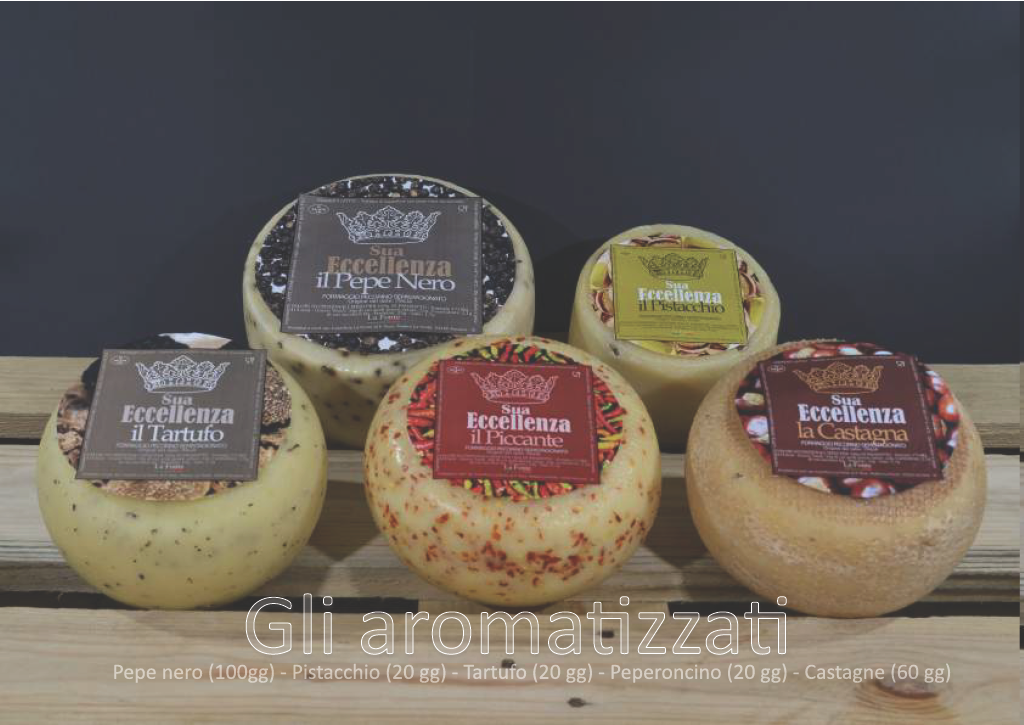
\includegraphics{../../img/LaFonte_gliaromatizzati1024_1.png}

}

\end{minipage}%

\end{table}

\renewcommand{\arraystretch}{1.6}

\begin{table}

\caption{\label{tbl-panel-aff-grare}Caseificio La Fonte (Asciano -
Siena)}\begin{minipage}[t]{0.60\linewidth}
\subcaption{\label{tbl-panel-aff-grare-1}Gli Affinati }

\tabularnewline

\fontsize{9.5}{11.5}\selectfont
\begin{tabular}{>{\raggedright\arraybackslash}p{3.25cm}>{\raggedright\arraybackslash}p{2.25cm}l}
\toprule
\textbf{Prodotto} & \textbf{Quantità} & \textbf{CHF/Kg}\\
\midrule
\textbf{\em{Gli Affinati di La Fonte}} & \textbf{Una forma 1,5-3 kg} & \textbf{}\\
\cmidrule{1-3}
 & < 10 kg & 38.7\\

\multirow[t]{-2}{3.25cm}{\raggedright\arraybackslash \em{Sua Eccellenza Il Foglia di Noce (90gg)}} & > 10kg & 34.8\\
\cmidrule{1-3}
 & < 10 kg & 39.2\\

\multirow[t]{-2}{3.25cm}{\raggedright\arraybackslash \em{Sua Eccellenza Il Re Fieno (70gg)}} & > 10kg & 35.2\\
\cmidrule{1-3}
 & < 10 kg & 38.7\\

\multirow[t]{-2}{3.25cm}{\raggedright\arraybackslash \em{Sua Eccellenza Il Germe di grano (60+45gg)}} & > 10kg & 34.8\\
\cmidrule{1-3}
 & < 10 kg & 38.7\\

\multirow[t]{-2}{3.25cm}{\raggedright\arraybackslash \em{Sua Eccellenza Le Vinacce (90+4gg)}} & > 10kg & 34.8\\
\cmidrule{1-3}
 & < 10 kg & 38.7\\

\multirow[t]{-2}{3.25cm}{\raggedright\arraybackslash \em{Sua Eccellenza Il Peparello (90gg)}} & > 10kg & 34.8\\
\bottomrule
\multicolumn{3}{l}{\rule{0pt}{1em}\textit{Note: }}\\
\multicolumn{3}{l}{\rule{0pt}{1em}gg: Giorni Stagionatura}\\
\multicolumn{3}{l}{\rule{0pt}{1em}}\\
\end{tabular}

\end{minipage}%
%
\begin{minipage}[t]{0.40\linewidth}

\raisebox{-\height}{

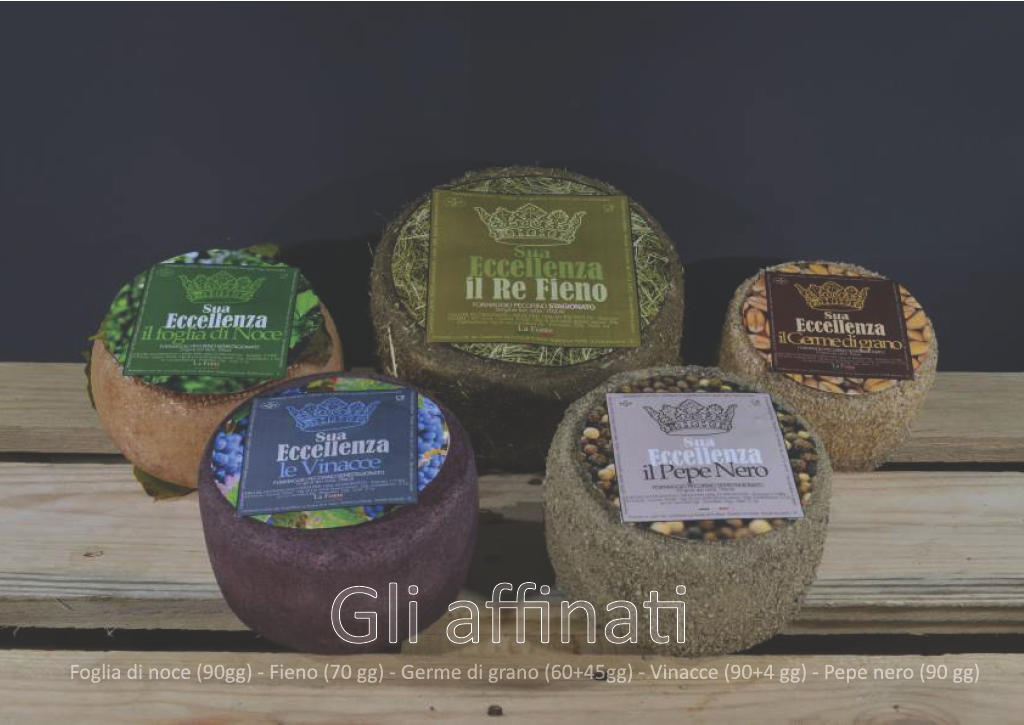
\includegraphics{../../img/LaFonte_GliAffinati1024_1.png}

}

\end{minipage}%
\newline
\begin{minipage}[t]{0.60\linewidth}
\subcaption{\label{tbl-panel-aff-grare-2}Il Grande ed i Re }

\tabularnewline

\fontsize{9.5}{11.5}\selectfont
\begin{tabular}{>{\raggedright\arraybackslash}p{3.25cm}>{\raggedright\arraybackslash}p{2.25cm}l}
\toprule
\textbf{Prodotto} & \textbf{Quantità} & \textbf{CHF/Kg}\\
\midrule
\textbf{\em{Il Grande e i Re}} & \textbf{Una forma 1,5-3 kg} & \textbf{}\\
\cmidrule{1-3}
 & < 10 kg & 38.5\\

\multirow[t]{-2}{3.25cm}{\raggedright\arraybackslash \em{Sua Eccellenza Il Grande (90gg)}} & > 10kg & 34.6\\
\cmidrule{1-3}
 & < 10 kg & 47\\

\multirow[t]{-2}{3.25cm}{\raggedright\arraybackslash \em{Sua Eccellenza Il Re Sole (200gg)}} & > 10kg & 42.3\\
\cmidrule{1-3}
 & < 10 kg & 39.4\\

\multirow[t]{-2}{3.25cm}{\raggedright\arraybackslash \em{Sua Eccellenza Il Re Grotta (90+60gg)}} & > 10kg & 35.5\\
\bottomrule
\multicolumn{3}{l}{\rule{0pt}{1em}\textit{Note: }}\\
\multicolumn{3}{l}{\rule{0pt}{1em}gg: Giorni Stagionatura}\\
\multicolumn{3}{l}{\rule{0pt}{1em}}\\
\end{tabular}

\end{minipage}%
%
\begin{minipage}[t]{0.40\linewidth}

\raisebox{-\height}{

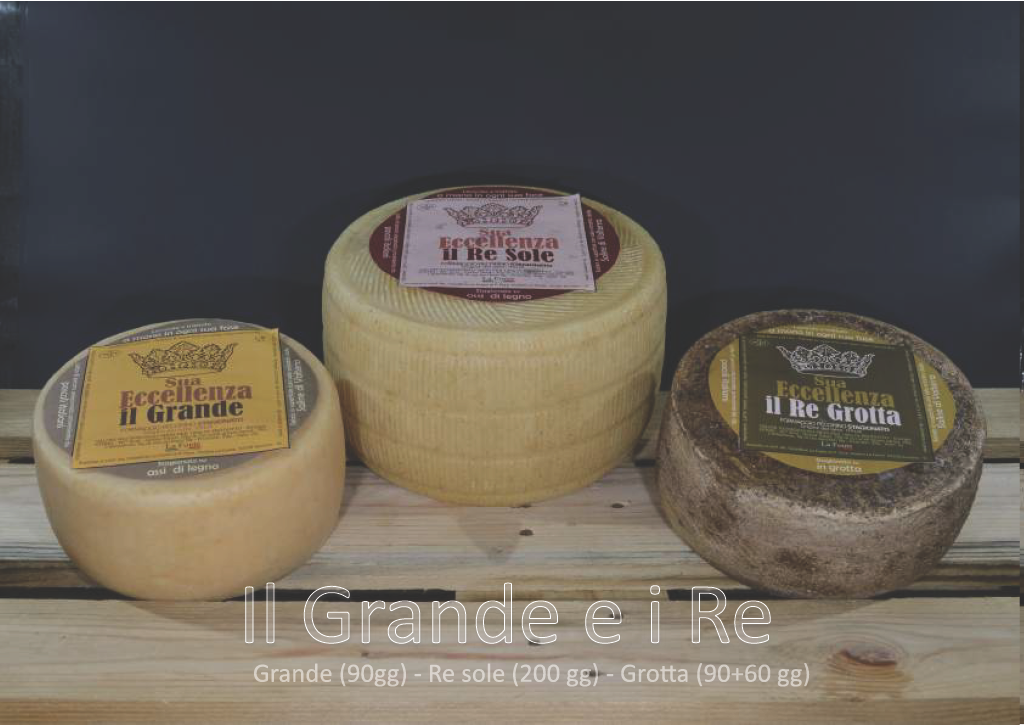
\includegraphics{../../img/IlGrande1024_1.png}

}

\end{minipage}%

\end{table}

\renewcommand{\arraystretch}{1.6}

\begin{table}

\caption{\label{tbl-panel-latt}Caseificio La Fonte (Asciano -
Siena)}\begin{minipage}[t]{0.60\linewidth}
\subcaption{\label{tbl-panel-latt-1}Linea Latte di Siena }

\tabularnewline

\fontsize{9.5}{11.5}\selectfont
\begin{tabular}{>{\raggedright\arraybackslash}p{3.25cm}>{\raggedright\arraybackslash}p{2.25cm}l}
\toprule
\textbf{Prodotto} & \textbf{Quantità} & \textbf{CHF/Kg}\\
\midrule
\textbf{\em{Linea Latte di Siena}} & \textbf{Una forma 1,5-5 kg} & \textbf{}\\
\cmidrule{1-3}
 & < 10 kg & 34.2\\

\multirow[t]{-2}{3.25cm}{\raggedright\arraybackslash \em{Cecco Latte Siena (20gg)}} & > 10kg & 30.8\\
\cmidrule{1-3}
 & < 10 kg & 35.2\\

\multirow[t]{-2}{3.25cm}{\raggedright\arraybackslash \em{Nobile Latte Siena (40gg)}} & > 10kg & 31.7\\
\cmidrule{1-3}
 & < 10 kg & 36.8\\

\multirow[t]{-2}{3.25cm}{\raggedright\arraybackslash \em{Mangia Latte Siena (70gg)}} & > 10kg & 33.1\\
\cmidrule{1-3}
 & < 10 kg & 37.8\\

\multirow[t]{-2}{3.25cm}{\raggedright\arraybackslash \em{Balzana Latte Siena (60gg)}} & > 10kg & 34\\
\cmidrule{1-3}
 & < 10 kg & 40.3\\

\multirow[t]{-2}{3.25cm}{\raggedright\arraybackslash \em{Tolomeo Latte Siena (90gg)}} & > 10kg & 36.3\\
\cmidrule{1-3}
 & < 10 kg & 41\\

\multirow[t]{-2}{3.25cm}{\raggedright\arraybackslash \em{Fieno Latte Siena (70gg)}} & > 10kg & 36.9\\
\bottomrule
\multicolumn{3}{l}{\rule{0pt}{1em}\textit{Note: }}\\
\multicolumn{3}{l}{\rule{0pt}{1em}gg: Giorni Stagionatura}\\
\multicolumn{3}{l}{\rule{0pt}{1em}}\\
\end{tabular}

\end{minipage}%
%
\begin{minipage}[t]{0.40\linewidth}

\raisebox{-\height}{

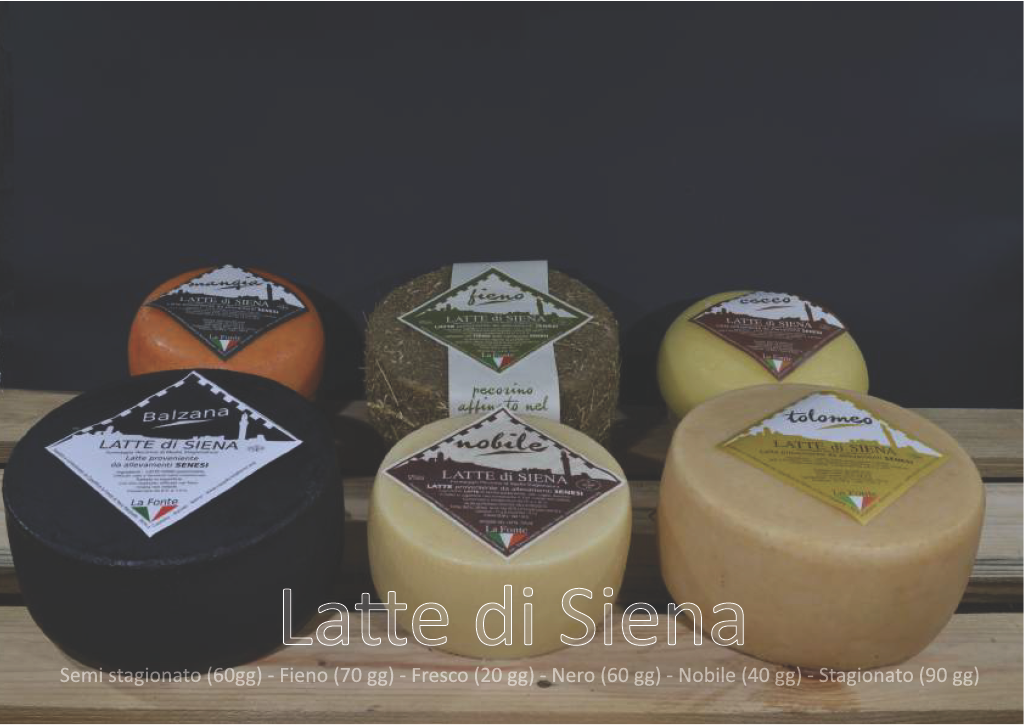
\includegraphics{../../img/Latte_di_siena1024_1.png}

}

\end{minipage}%

\end{table}

\begin{table}

\caption{\label{tbl-panel-mmons}Salumeria di Monte San
Savino}\begin{minipage}[t]{0.60\linewidth}
\subcaption{\label{tbl-panel-mmons-1}Porchette }

\tabularnewline

\fontsize{9.5}{11.5}\selectfont
\begin{tabular}{>{\raggedright\arraybackslash}p{3.25cm}>{\raggedright\arraybackslash}p{2.25cm}l}
\toprule
\textbf{Prodotto} & \textbf{Quantità} & \textbf{CHF/Kg}\\
\midrule
\textbf{\em{Porchetta}} & \textbf{8-11 Kg} & \textbf{}\\
\cmidrule{1-3}
 & 1/2 o 1 & 42.1\\

\multirow[t]{-2}{3.25cm}{\raggedright\arraybackslash \em{Tronchetto Cotto a Legna}} & >1 & 37.5\\
\bottomrule
\multicolumn{3}{l}{\rule{0pt}{1em}\textit{Note: }}\\
\multicolumn{3}{l}{\rule{0pt}{1em}Quantità indica il peso di un pezzo}\\
\multicolumn{3}{l}{\rule{0pt}{1em}}\\
\end{tabular}

\end{minipage}%
%
\begin{minipage}[t]{0.40\linewidth}

\raisebox{-\height}{

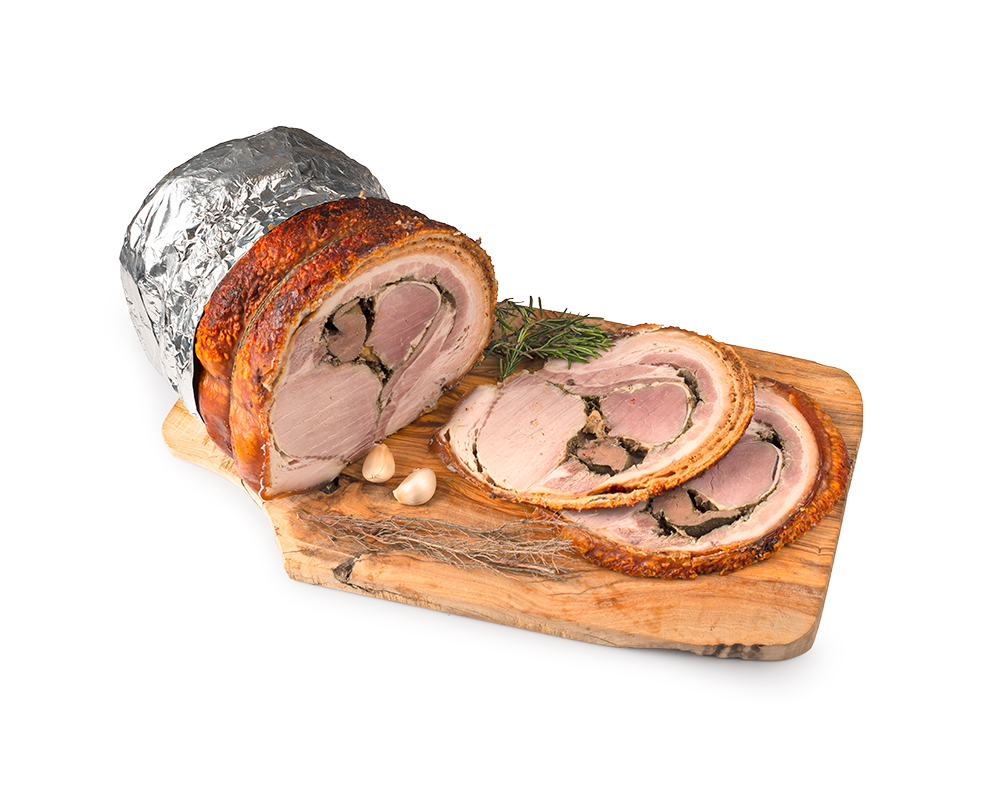
\includegraphics{../../img/Tronchetto-cotto-a-legna.jpg}

}

\end{minipage}%
\newline
\begin{minipage}[t]{0.60\linewidth}
\subcaption{\label{tbl-panel-mmons-2}Finocchione }

\tabularnewline

\fontsize{9.5}{11.5}\selectfont
\begin{tabular}{>{\raggedright\arraybackslash}p{3.25cm}>{\raggedright\arraybackslash}p{2.25cm}l}
\toprule
\textbf{Prodotto} & \textbf{Quantità} & \textbf{CHF/Kg}\\
\midrule
\textbf{\em{Finocchiona}} & \textbf{10-12 kg} & \textbf{}\\
\cmidrule{1-3}
 & 1/2 o 1 & 40.5\\

\multirow[t]{-2}{3.25cm}{\raggedright\arraybackslash \em{Finocchiona IGP}} & >1 & 36.2\\
\bottomrule
\multicolumn{3}{l}{\rule{0pt}{1em}\textit{Note: }}\\
\multicolumn{3}{l}{\rule{0pt}{1em}Quantità indica il peso di un pezzo}\\
\multicolumn{3}{l}{\rule{0pt}{1em}}\\
\end{tabular}

\end{minipage}%
%
\begin{minipage}[t]{0.40\linewidth}

\raisebox{-\height}{

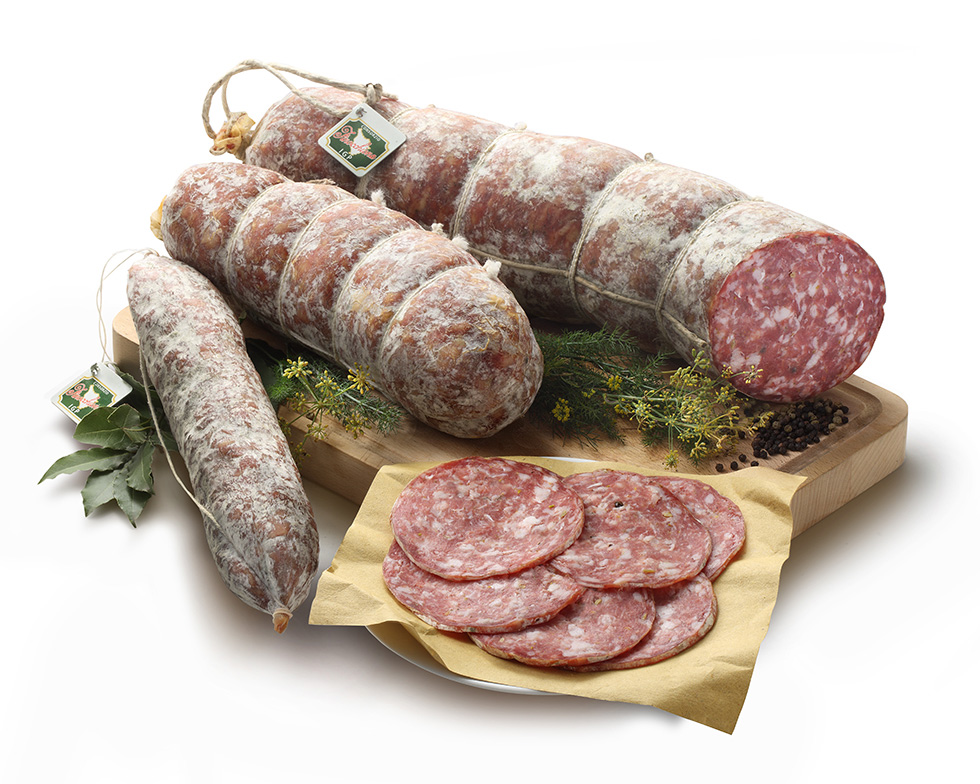
\includegraphics{../../img/Finocchiona-IGP.jpg}

}

\end{minipage}%

\end{table}

\begin{table}

\caption{\label{tbl-panel-luca}I Sughi di Luca (Monte
Amiata)}\begin{minipage}[t]{0.60\linewidth}
\subcaption{\label{tbl-panel-luca-1}Sughi / Zuppe / Pate\textquotesingle{} }

\tabularnewline

\fontsize{9.5}{11.5}\selectfont
\begin{tabular}{>{\raggedright\arraybackslash}p{3.25cm}>{\raggedright\arraybackslash}p{2.25cm}l}
\toprule
\textbf{Prodotto} & \textbf{Quantità} & \textbf{CHF}\\
\midrule
\textbf{\em{Sughi di Luca}} & \textbf{Barattolo Vetro} & \textbf{}\\
\cmidrule{1-3}
 & <10 & 8.8\\

\multirow[t]{-2}{3.25cm}{\raggedright\arraybackslash \em{Sugo Aglione (300gr)}} & >=10 & 8.1\\
\cmidrule{1-3}
 & <10 & 9.1\\

\multirow[t]{-2}{3.25cm}{\raggedright\arraybackslash \em{Ribollita (300gr)}} & >=10 & 8.4\\
\cmidrule{1-3}
 & <10 & 10.1\\

\multirow[t]{-2}{3.25cm}{\raggedright\arraybackslash \em{Scottiglia (300gr)}} & >=10 & 9.2\\
\cmidrule{1-3}
 & <10 & 10.6\\

\multirow[t]{-2}{3.25cm}{\raggedright\arraybackslash \em{Sugo Cinghiale (300gr)}} & >=10 & 9.7\\
\cmidrule{1-3}
 & <10 & 10.6\\

\multirow[t]{-2}{3.25cm}{\raggedright\arraybackslash \em{Cinta Senese e Porri (300gr)}} & >=10 & 9.7\\
\bottomrule
\multicolumn{3}{l}{\rule{0pt}{1em}\textit{Note: }}\\
\multicolumn{3}{l}{\rule{0pt}{1em}Barattoli in vetro (300gr), scadenza 3 mesi}\\
\multicolumn{3}{l}{\rule{0pt}{1em}}\\
\end{tabular}

\end{minipage}%
%
\begin{minipage}[t]{0.40\linewidth}

\raisebox{-\height}{

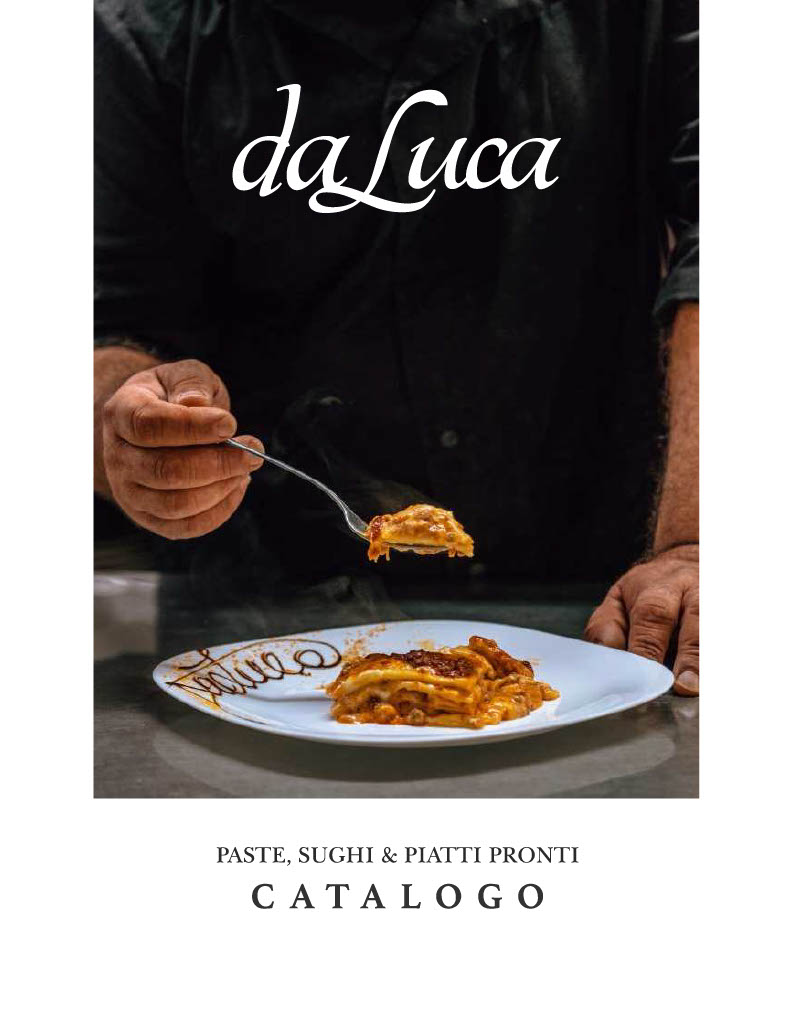
\includegraphics{../../img/I_Sugh_d_Luca.jpg}

}

\end{minipage}%
\newline
\begin{minipage}[t]{0.60\linewidth}
\subcaption{\label{tbl-panel-luca-2}  }

\tabularnewline

\fontsize{9.5}{11.5}\selectfont
\begin{tabular}{>{\raggedright\arraybackslash}p{3.25cm}>{\raggedright\arraybackslash}p{2.25cm}l}
\toprule
\textbf{Prodotto} & \textbf{Quantità} & \textbf{CHF}\\
\midrule
\textbf{\em{Pate' di Luca}} & \textbf{Barattolo Vetro} & \textbf{}\\
\cmidrule{1-3}
 & <10 & 7.1\\

\multirow[t]{-2}{3.25cm}{\raggedright\arraybackslash \em{Pate' Fegatini (200gr)}} & >=10 & 6.5\\
\bottomrule
\multicolumn{3}{l}{\rule{0pt}{1em}\textit{Note: }}\\
\multicolumn{3}{l}{\rule{0pt}{1em}Barattoli in vetro (200gr), scadenza 3 mesi}\\
\multicolumn{3}{l}{\rule{0pt}{1em}}\\
\end{tabular}

\end{minipage}%
%
\begin{minipage}[t]{0.40\linewidth}

\raisebox{-\height}{

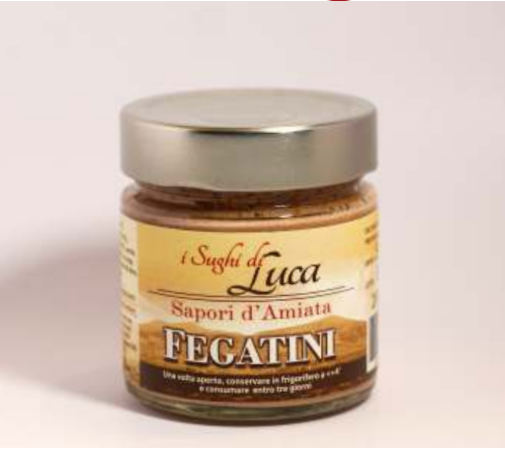
\includegraphics{../../img/Pate_Fegatini_daluca.png}

}

\end{minipage}%

\end{table}



\end{document}
